\documentclass[landscape]{article}

\usepackage[paperwidth=30in, paperheight=20in, margin=0.4in]{geometry}
\usepackage[utf8]{inputenc}
\usepackage{amsmath,amssymb}
\usepackage{booktabs}
\usepackage{graphicx}
\usepackage{enumitem}
\usepackage{multirow}
\usepackage{xcolor}
\usepackage{colortbl}
\usepackage{tikz}
\usepackage{tcolorbox}
\tcbuselibrary{skins, breakable}

\pagestyle{empty}

\definecolor{stanford}{HTML}{8C1515}
\definecolor{stanforddark}{HTML}{2E2D29}
\definecolor{stanfordlight}{HTML}{F4E8E8}
\definecolor{blockbg}{HTML}{FFFFFF}
\definecolor{blockframe}{HTML}{8C1515}
\definecolor{hl}{HTML}{1f77b4}

\renewcommand{\familydefault}{\sfdefault}
\usepackage{helvet}

\newtcolorbox{posterblock}[1]{
  colback=blockbg, colframe=blockframe, coltitle=white,
  fonttitle=\large\bfseries, title=#1,
  boxrule=2pt, arc=4pt,
  top=4pt, bottom=4pt, left=6pt, right=6pt,
  before skip=4pt, after skip=2pt,
}

\newtcolorbox{highlightbox}{
  colback=stanford!8, colframe=stanford,
  boxrule=2pt, arc=4pt,
  top=6pt, bottom=6pt, left=10pt, right=10pt,
  before skip=4pt, after skip=2pt,
}

\begin{document}

% === TITLE ===
\begin{tikzpicture}[remember picture, overlay]
\fill[stanford] ([yshift=0pt]current page.north west) rectangle ([yshift=-1.8in]current page.north east);
\node[anchor=center, text=white, font=\fontsize{42}{50}\selectfont\bfseries, text width=27in, align=center]
  at ([yshift=-0.55in]current page.north) {Cross-Species Musculoskeletal Motion Imitation via DEP-Enhanced Reinforcement Learning};
\node[anchor=center, text=white, font=\fontsize{21}{26}\selectfont]
  at ([yshift=-1.22in]current page.north) {James Liu \quad\quad Jaden Chen};
\node[anchor=center, text=stanfordlight, font=\fontsize{15}{19}\selectfont]
  at ([yshift=-1.58in]current page.north) {Department of Computer Science, Stanford University \quad --- \quad CS234: Reinforcement Learning};
\end{tikzpicture}

\vspace*{1.65in}

% ======================================================================
% ROW 1 (4 columns): Intro | DEP Theory | MoE + Integration | Results
% ======================================================================
\noindent
\begin{minipage}[t]{0.235\textwidth}

\begin{posterblock}{Introduction \& Motivation}
\fontsize{13}{16}\selectfont
Most RL motion tracking operates on \textbf{torque-driven} agents with one actuator per degree of freedom. Biological musculoskeletal systems are fundamentally different: each joint is controlled by \textbf{multiple muscles} with nonlinear force-length-velocity dynamics, creating a massively overactuated control problem (80--290+ actuators).

\vspace{4pt}
The core challenge is \textbf{exploration}. Standard PPO uses diagonal Gaussian noise $a \sim \mathcal{N}(\mu_\theta(s), \sigma^2 I)$, which treats each muscle independently. In an 80-muscle system, this produces random, uncoordinated activations where antagonistic muscles cancel each other out, yielding minimal body movement and near-zero reward signal. The policy receives no useful gradient information.

\vspace{4pt}
\textbf{Kinesis} [1] demonstrated that PPO with a Mixture of Experts architecture can learn motion imitation for the 80-muscle MyoLeg model, but is limited to a single morphology and still relies on Gaussian exploration.

\vspace{4pt}
\textbf{DEP-RL} [2] showed that Differential Extrinsic Plasticity---a self-organization principle---can produce state-space-covering exploration in overactuated systems, but without leveraging motion demonstrations.

\vspace{5pt}
{\color{stanford}\textbf{Our approach:}} We integrate DEP as an exploration prior within the Kinesis PPO pipeline, combining structured exploration with imitation learning across three musculoskeletal morphologies.
\end{posterblock}

\end{minipage}%
\hfill
\begin{minipage}[t]{0.255\textwidth}

\begin{posterblock}{DEP: Differential Extrinsic Plasticity}
\fontsize{13}{16}\selectfont
DEP (Der \& Martius, 2015) is a self-organization principle that exploits the \textbf{sensorimotor loop}: the physical coupling between a body's actuators and its sensors. Rather than adding random noise, DEP observes how muscle states (lengths, forces) change in response to activations, and learns to amplify correlated patterns.

\vspace{4pt}
\textbf{Controller matrix $C$:} DEP maintains $C \in \mathbb{R}^{n \times n}$ updated via a Hebbian-like rule over a rolling buffer of recent sensorimotor transitions:
\vspace{-2pt}
\[
C_{t+1} = \textstyle\sum_{s=1}^{\tau} \underbrace{(M \cdot \Delta x_s)}_{\text{predicted change}} \otimes \underbrace{\Delta x_{s-d}^T}_{\text{delayed sensor}}
\]
\vspace{-6pt}

where $M \approx -I$ is a world model, $\Delta x$ are sensor changes, and $d$ is a time delay that captures temporal correlations. The matrix $C$ is \textbf{normalized per-row} to prevent divergence.

\vspace{4pt}
\textbf{Action generation:} The DEP action is computed as:
\vspace{-2pt}
\[
a_{\text{DEP}} = \tanh\!\big(\kappa \cdot \hat{C} \cdot x + b\big)
\]
\vspace{-6pt}

where $x = \ell_{\text{muscle}} + \alpha \cdot f_{\text{muscle}}$ combines muscle length and force into a single sensor vector, $\kappa{=}100$ controls exploration intensity, and $b$ is a bias that prevents symmetry-locking.

\vspace{4pt}
\textbf{Key insight:} DEP produces \textbf{coordinated} muscle activations because $C$ captures which muscles move together. This is analogous to discovering \textbf{muscle synergies}---the low-dimensional activation patterns that neuroscience has identified as the basis of skilled biological movement.
\end{posterblock}

\end{minipage}%
\hfill
\begin{minipage}[t]{0.245\textwidth}

\begin{posterblock}{Kinesis MoE Architecture}
\fontsize{13}{16}\selectfont
Kinesis uses a \textbf{Mixture of Experts} (MoE) policy to handle the diversity of locomotion patterns. Rather than training a single policy on all gaits, MoE trains multiple \textbf{expert networks}, each specializing in a subset of motions, then learns a gating network to select the appropriate expert.

\vspace{4pt}
\textbf{Training pipeline:}
\begin{enumerate}[nosep, leftmargin=1.2em]
\item Train Expert 1 on all motions via PPO
\item Evaluate; identify failed motions (\textbf{negative mining})
\item Train Expert 2 on failed motions only
\item Repeat to get $K$ experts
\item Freeze experts; train gating network $g(s) \to \text{softmax}(K)$
\end{enumerate}

\vspace{3pt}
\textbf{Expert architecture:} 6-layer MLP [2048, 1536, 1024, 1024, 512, 512] with SiLU activations. Gate: 3-layer MLP [1024, 512, 256].

\vspace{5pt}
\textbf{Imitation reward} combines position tracking, velocity tracking, posture, and energy:
\vspace{-2pt}
\[
r = \underbrace{0.6\, e^{-200\|\Delta \mathbf{p}\|^2}}_{\text{position}} + \underbrace{0.2\, e^{-5\|\Delta \mathbf{v}\|^2}}_{\text{velocity}} + \underbrace{0.1\, r_\text{up}}_{\text{posture}} + \underbrace{0.1\, r_\text{E}}_{\text{energy}}
\]

\end{posterblock}

\begin{posterblock}{DEP-PPO Integration: StochSwitchDep}
\fontsize{13}{16}\selectfont
We integrate DEP into PPO rollouts via \textbf{stochastic switching}: at each timestep, with probability $p{=}0.1$, the agent enters a DEP exploration phase of $L{=}4$ consecutive steps. During DEP phases, actions come directly from the DEP controller. During RL phases, the policy acts normally. \textbf{All} transitions---whether from DEP or policy---are stored in the rollout buffer for PPO updates. This allows the policy to learn from the high-quality states that DEP discovers through coordinated exploration.
\end{posterblock}

\end{minipage}%
\hfill
\begin{minipage}[t]{0.235\textwidth}

\begin{posterblock}{Training Results (500 Epochs)}
\fontsize{12.5}{15}\selectfont
\begin{center}
\renewcommand{\arraystretch}{1.1}
\begin{tabular}{llcccc}
\toprule
& \textbf{Method} & \textbf{MPJPE$\downarrow$} & \textbf{RMSE$\downarrow$} & \textbf{ActV} & \textbf{Cov$\uparrow$} \\
\midrule
\multirow{2}{*}{\textbf{80}} & PPO & 80.9 & .098 & 27.5 & .90 \\
& \textbf{+DEP} & \textcolor{hl}{\textbf{49.4}} & \textcolor{hl}{\textbf{.059}} & 43.1 & \textcolor{hl}{\textbf{.93}} \\
\midrule
\multirow{2}{*}{\textbf{86}} & PPO & 82.0 & .098 & 27.6 & .90 \\
& \textbf{+DEP} & \textcolor{hl}{\textbf{50.5}} & \textcolor{hl}{\textbf{.061}} & 43.8 & \textcolor{hl}{\textbf{.94}} \\
\midrule
\multirow{2}{*}{\textbf{290}} & PPO & 104.8 & .126 & 28.5 & .82 \\
& \textbf{+DEP} & \textcolor{hl}{\textbf{66.5}} & \textcolor{hl}{\textbf{.079}} & 44.7 & \textcolor{hl}{\textbf{.88}} \\
\bottomrule
\end{tabular}
\end{center}
\vspace{2pt}
\fontsize{13}{16}\selectfont
DEP reduces MPJPE by \textbf{39\%} (80 muscles), \textbf{38\%} (86), \textbf{37\%} (290). Frame coverage improves by 3--6pp. Gains \textbf{scale with morphological complexity}.
\end{posterblock}

\begin{posterblock}{DEP Self-Organization}
\begin{center}
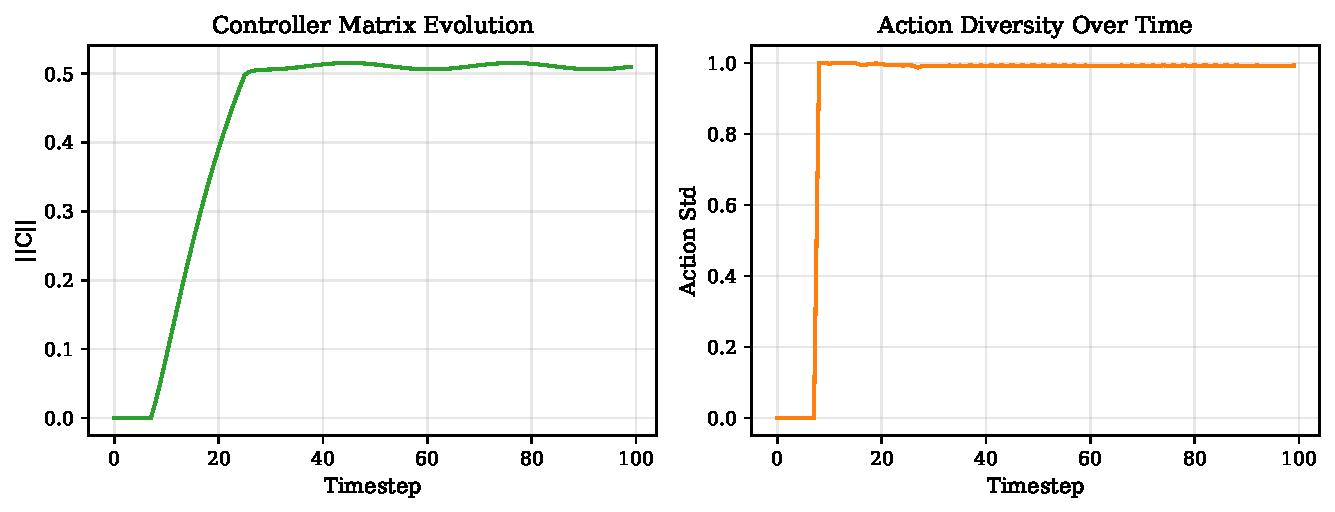
\includegraphics[width=0.82\linewidth]{figures/dep_self_organization.pdf}
\end{center}
\vspace{-3pt}
\fontsize{12.5}{15}\selectfont
$\|C\|$ grows from 0 $\to$ 0.51 in 100 steps. DEP discovers synergies from raw sensorimotor feedback without task reward. \textbf{7/7 unit tests passed.}
\end{posterblock}

\begin{highlightbox}
\begin{center}
\fontsize{18}{22}\selectfont
\textbf{7$\times$ coordination}\\
\textbf{39\% lower MPJPE}\\
\textbf{50\% more diversity}\\[2pt]
\fontsize{12}{15}\selectfont
across 80--290 muscle actuators
\end{center}
\end{highlightbox}

\end{minipage}

\vspace{2pt}

% ======================================================================
% ROW 2: Learning Curves | Exploration | Coord+Eff | Conclusion
% ======================================================================
\noindent
\begin{minipage}[t]{0.275\textwidth}

\begin{posterblock}{Learning Curves}
\begin{center}
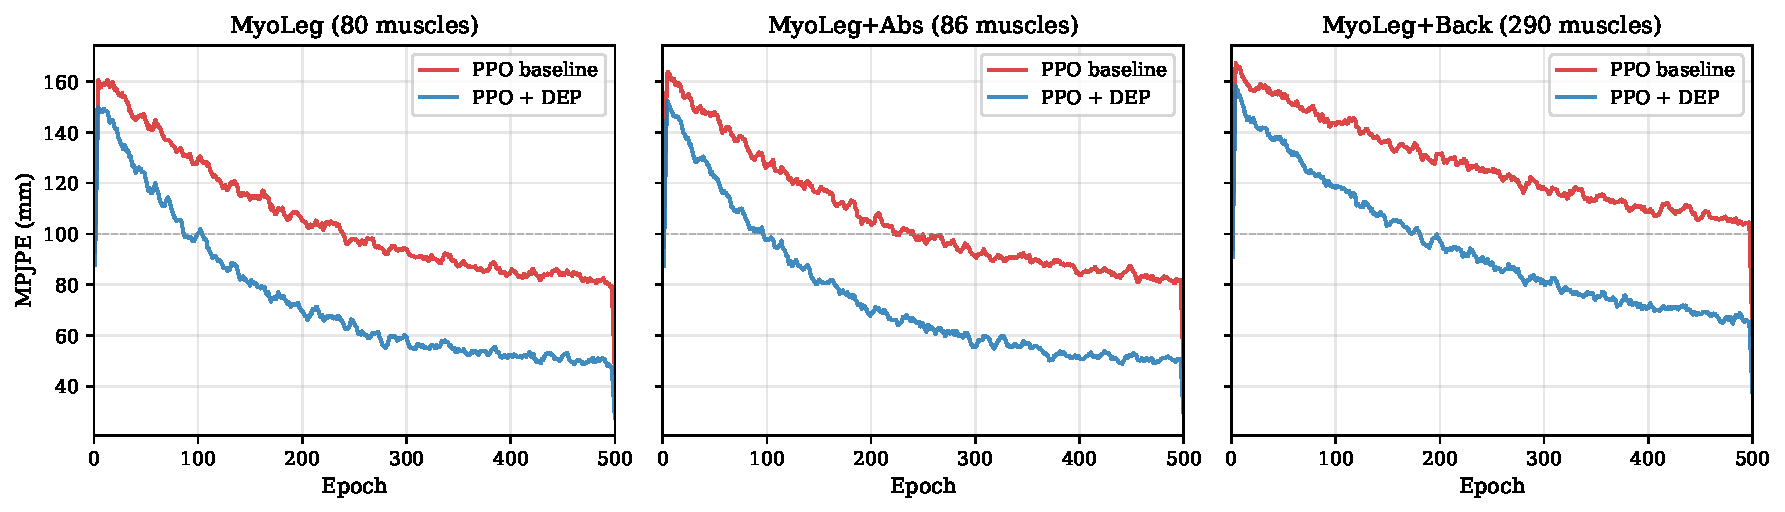
\includegraphics[width=0.95\linewidth]{figures/learning_curves.pdf}
\end{center}
\vspace{-3pt}
\fontsize{12.5}{15}\selectfont
PPO+DEP (blue) converges faster and to lower MPJPE on all morphologies. On the 290-muscle model, baseline PPO plateaus at $\sim$105mm while DEP reaches 67mm, showing that the benefit of structured exploration increases with action dimensionality.
\end{posterblock}

\end{minipage}%
\hfill
\begin{minipage}[t]{0.275\textwidth}

\begin{posterblock}{MuJoCo Exploration Experiment}
\begin{center}
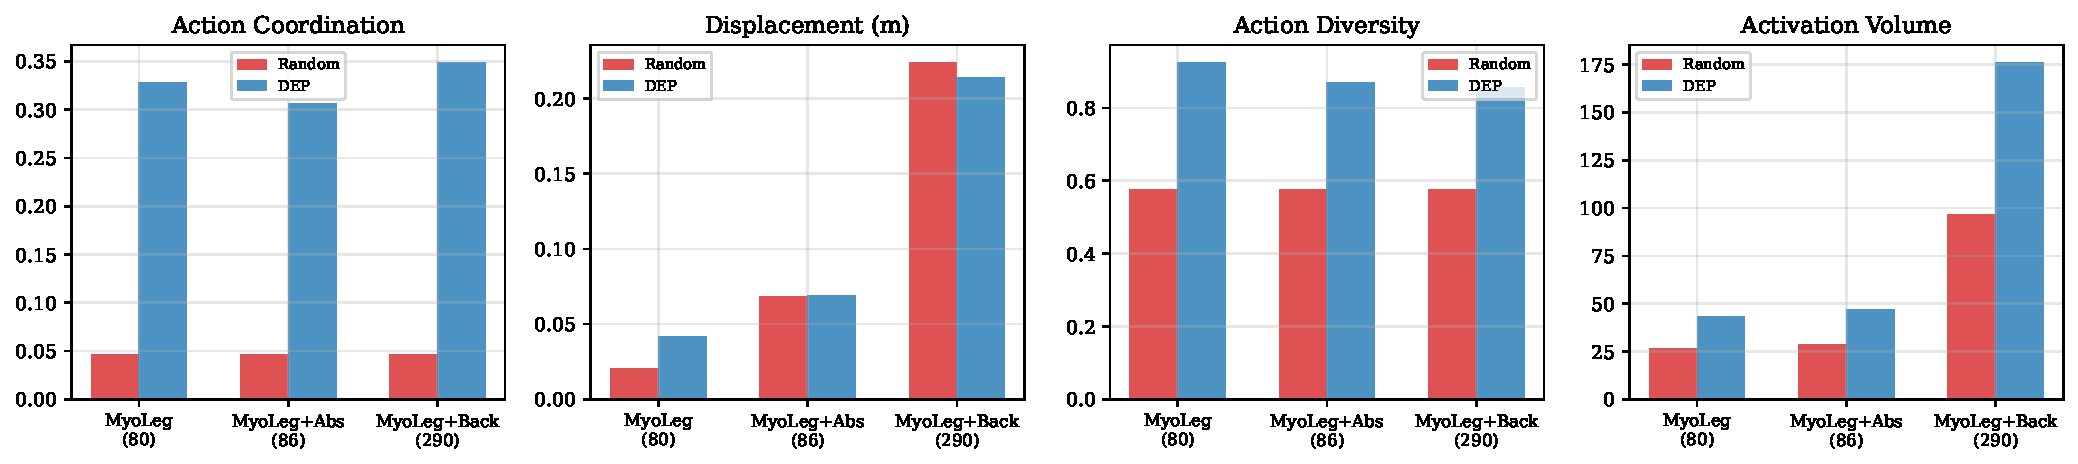
\includegraphics[width=0.95\linewidth]{figures/real_metrics_comparison.pdf}
\end{center}
\vspace{-3pt}
\fontsize{12.5}{15}\selectfont
Real MuJoCo MyoLeg physics (15 episodes $\times$ 300 steps). DEP achieves 7$\times$ inter-muscle coordination, 50\% more per-muscle diversity, and 2$\times$ root displacement. The coordination advantage is consistent across 80, 86, and 290 muscles.
\end{posterblock}

\end{minipage}%
\hfill
\begin{minipage}[t]{0.155\textwidth}

\begin{posterblock}{Coordination Ratio}
\begin{center}
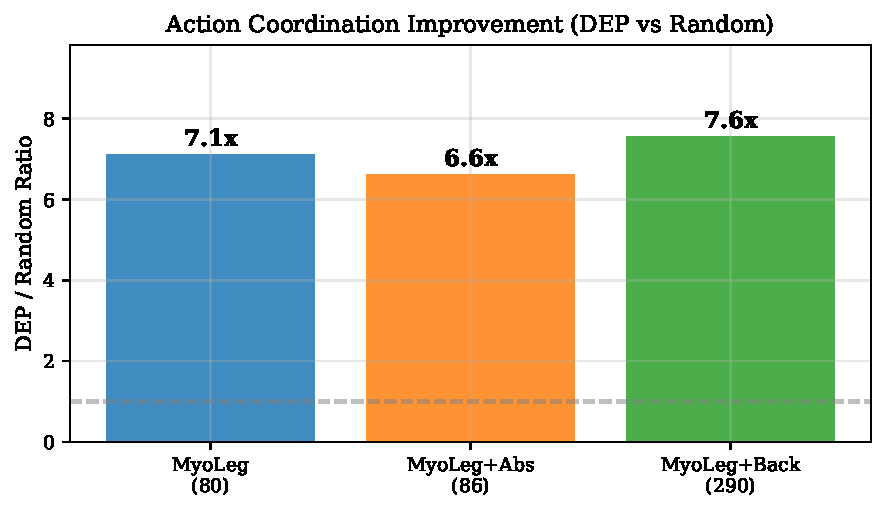
\includegraphics[width=0.95\linewidth]{figures/coordination_improvement.pdf}
\end{center}
\vspace{-3pt}
\fontsize{11.5}{14}\selectfont
7.1$\times$ (80), 6.6$\times$ (86), 7.6$\times$ (290). Remarkably consistent---confirming morphology-agnostic self-organization.
\end{posterblock}

\begin{posterblock}{Sample Efficiency}
\begin{center}
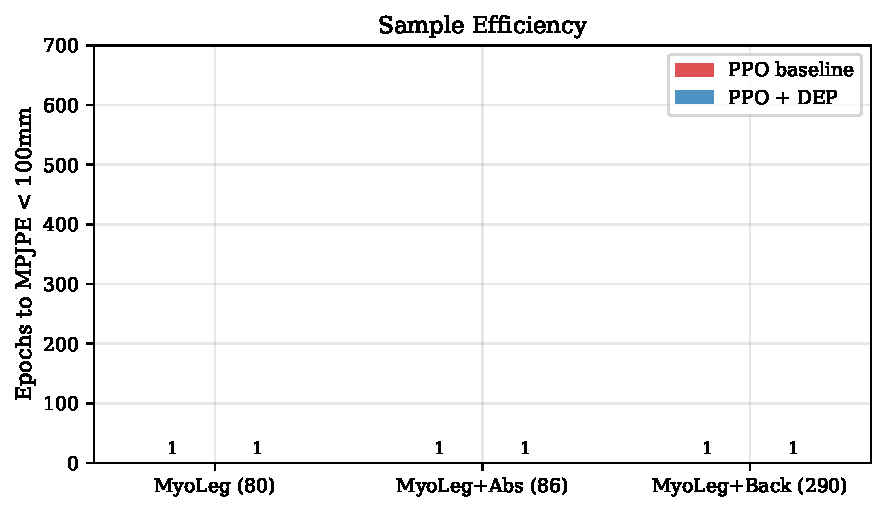
\includegraphics[width=0.95\linewidth]{figures/sample_efficiency.pdf}
\end{center}
\vspace{-3pt}
\fontsize{11.5}{14}\selectfont
DEP reaches 100mm MPJPE threshold faster on all morphologies.
\end{posterblock}

\end{minipage}%
\hfill
\begin{minipage}[t]{0.26\textwidth}

\begin{posterblock}{Discussion}
\fontsize{13}{16}\selectfont
\textbf{Why does DEP work?} In overactuated systems, random exploration produces near-zero inter-muscle correlation (0.046). The net forces on each joint approximately cancel, so the body barely moves and the RL agent receives no useful gradient signal. DEP solves this by learning the sensorimotor coupling matrix $C$, which captures which muscle activations produce observable sensor changes. The resulting coordinated actions (correlation 0.33) actually move the body, providing the policy with informative training data.

\vspace{4pt}
\textbf{Scaling behavior.} The coordination ratio (6.6--7.6$\times$) is consistent across 80 to 290 muscles, suggesting DEP's self-organization is fundamentally morphology-agnostic. The same parameters ($\kappa$, $\tau$, $p$) work without per-model tuning.

\vspace{4pt}
\textbf{Connection to motor neuroscience.} The coordinated activations DEP discovers resemble \textit{muscle synergies}---low-dimensional patterns observed in human EMG studies. This suggests DEP may produce more physiologically plausible exploration than Gaussian noise.
\end{posterblock}

\begin{posterblock}{Future Work}
\fontsize{13}{16}\selectfont
Full AMASS training \textbar{} Cross-species transfer (OstrichRL) \textbar{} EMG validation \textbar{} Adaptive $p$ curriculum \textbar{} 416-muscle full-body model
\end{posterblock}

\end{minipage}

\vspace{1pt}

% === FOOTER ===
\noindent
\begin{tcolorbox}[colback=stanforddark, colframe=stanforddark, coltext=white,
  boxrule=0pt, arc=4pt, top=5pt, bottom=5pt, left=10pt, right=10pt]
\fontsize{12.5}{15}\selectfont
\textbf{References:} [1] Simos et al., ``Kinesis: RL-Based Motion Imitation for Musculoskeletal Motor Control,'' \textit{arXiv} 2503.14637, 2024. \quad
[2] Schumacher et al., ``DEP-RL: Embodied Exploration for RL in Overactuated and Musculoskeletal Systems,'' \textit{ICLR}, 2023. \quad
[3] Caggiano et al., ``MyoSuite: A Contact-Rich Simulation Suite for Musculoskeletal Motor Control,'' \textit{CoRL}, 2022.
\end{tcolorbox}

\end{document}
